\documentclass[11pt, a4paper]{article}

\usepackage[margin=1in]{geometry} % manage page dimensions
\usepackage[utf8]{inputenc} % utf-8 encoding
\usepackage[italian]{babel} % italian default text
\usepackage[hidelinks]{hyperref} % link references
\usepackage{bookmark} % 
\usepackage{import} % import other .tex files
\usepackage{amsmath} % math commands
\usepackage{amssymb} % math symbols
\usepackage{amsthm} % math environments
\usepackage{amsmath} % equation align
\usepackage{siunitx} % SI unit
\usepackage{booktabs} % tabular enhance
\usepackage{multirow} % dynamic tabular cell dimensions
\usepackage{longtable} % multi-page table
\usepackage[labelfont=bf, skip=.5em, font=small]{caption} % beautiful caption
\usepackage{subcaption} % subfigure
\usepackage{graphicx} % import graphics
\usepackage{fancyhdr} % custom page header and footer

\graphicspath{{../assets/}} % base graphics path

\setlength{\parskip}{1em} % distance between paragraphs
\setlength{\parindent}{0em} % indentation at beginning of paragraph

\numberwithin{equation}{section} % equation tag relative to section

\title{Esperienza 3}
\author{Matteo Romano, Vittorio Strano}
\date{09/12/2021}

\begin{document}

\maketitle

\tableofcontents

\section{Obiettivo dell'esperienza}

Lo scopo dell'esperienza è quello di calcolare la frequenza di taglio di un circuito RC. Per farlo si analizza la differenza di potenziale ai capi di R (\autoref{fig:circuito R}) e/o ai capi di C (\autoref{fig:circuito C}) quando si sottopone il circuito ad una tensione variabile.

\begin{figure}[ht!]
    \centering
    \begin{subfigure}[c]{.3\textwidth}
        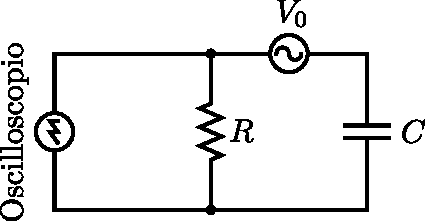
\includegraphics[width=\textwidth]{circuito_osc_R.pdf}
        \caption{Misure ai capi di R}
        \label{fig:circuito R}
    \end{subfigure}
    \hspace{1in}
    \begin{subfigure}[c]{.3\textwidth}
        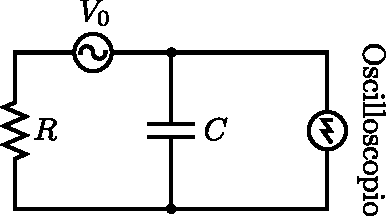
\includegraphics[width=\textwidth]{circuito_osc_C.pdf}
        \caption{Misure ai capi di C}
        \label{fig:circuito C}
    \end{subfigure}
    \caption{Schema circuito}
  \end{figure}

\section{Strumenti e materiali}

\begin{itemize}
    \item Generatore di tensione AC
    \item Multimetro digitale (utilizzato come ohmetro)
    \item Oscilloscopio
    \item Cavi
    \item Breadboard
    \item Resistore
    \item Condensatore
\end{itemize}

\section{Onda quadra} \label{sec:onda quadra}

La prima parte dell'esperimento consiste nell'applicare ai capi del circuito una tensione variabile secondo un'onda quadra di ampiezza picco-picco pari a \(V_{0}\). La frequenza dell'onda ($f = (3.46 \pm 0.06) \; kHz$) è stata scelta in modo da permettere al condensatore di completare il regime transitorio, passando da una tensione \(V_{0}/2\) fino ad una tensione \(- V_{0}/2\). La curva osservata nell'oscilloscopio rappresenta la tensione \(V_{C}\) ai capi del condensatore in funzione del tempo \(t\) e segue l'\autoref{eq:regime transitorio onda quadra}, dove con $\tau = RC$ si indica il tempo caratteristico del circuito.

\begin{equation} \label{eq:regime transitorio onda quadra}
    V_{C} = V_{0} \cdot e^{-t/\tau} - V_{0}/2
\end{equation}

Per prendere le misure il sistema di riferimento è stato traslato in modo da porre come zero delle ordinate il valore \(- V_{0}/2\) e ottenere l'\autoref{eq:regime transitorio condensatore}.

\begin{equation} \label{eq:regime transitorio condensatore}
    V = V_{0} \cdot e^{-t/\tau}
\end{equation}

Noto il valore di \(R = (1.874 \pm 0.004) \; \unit{k\Omega}\) (misurato con il multimetro) si vuole ottenere il valore di \(C\).

\subsection{Dati ed errori}

Sull'oscilloscopio è stato fissato il primo cursore in corrispondenza dell'asintoto della curva a \(- V_{0}/2\); questo sarà lo zero delle ordinate.

Il secondo cursore è stato fatto variare in modo da ottenere la differenza di potenziale al variare del tempo. Le misure ottenute sono riportate nella \autoref{tab:misure onda quadra} con i relativi errori pari a $1/10$ della scala.

\begin{table}[ht!]
    \centering
    \caption{Misure della variazione di tensione ai capi di $C$ nel regime transitorio}
    \import{../tables/}{onda_quadra_Vt.tex}
    \label{tab:misure onda quadra}
\end{table}

\subsection{Analisi dati}

\begin{equation*}
    V = V_{0} \cdot e^{-t/\tau} \implies \ln(V) = \ln(V_{0}) - \frac{t}{\tau}
\end{equation*}

Riportando le misure in un grafico semi-logaritmico (come in \autoref{fig:onda quadra pendenze}), ci si aspetta di ottenere una funzione lineare.

\begin{figure}[ht!]
    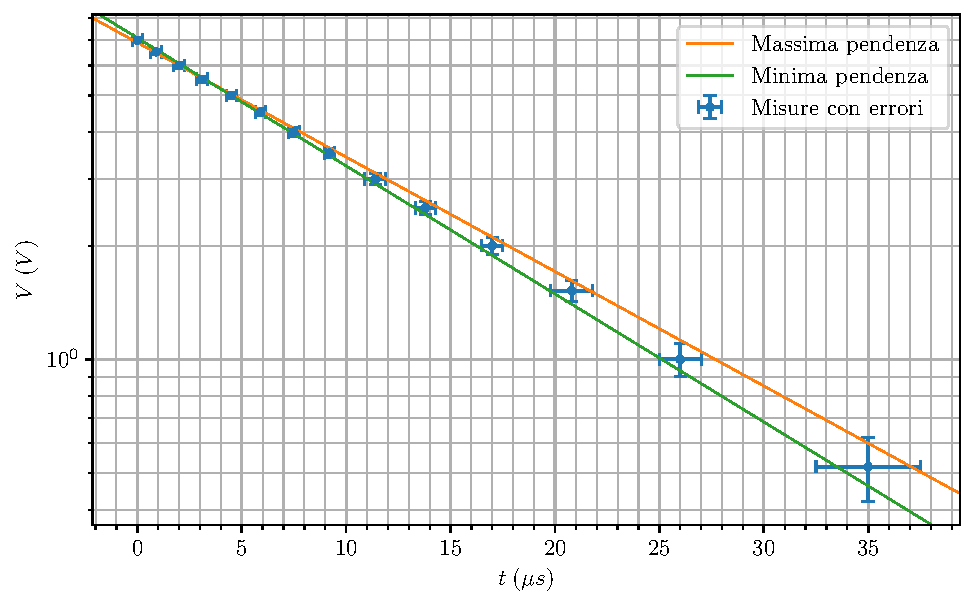
\includegraphics{onda_quadra_V(t)_pendenze.pdf}
    \caption{Grafico semi-logaritmico delle misure della variazione di tensione ai capi di $C$ nel regime transitorio}
    \label{fig:onda quadra pendenze}
\end{figure}

La retta di massima pendenza passa per i punti \((-0.2, 7)\) e \((35, 0.6)\), mentre la retta di minima pendenza passa per i punti \((0.2, 7)\) e \((34, 0.5)\).

\begin{equation*}
    m_{max} = \frac{\ln(7/0.6)}{- 0.2 - 35} = - 0.06979
    \qquad
    m_{min} = \frac{\ln(7/0.5)}{0.2 - 34} = - 0.07808
\end{equation*}

\begin{align*}
    m_{best} &= \frac{m_{max} + m_{min}}{2} = - 0.0739 \approx - 0.074 \\
    \delta m &= \frac{m_{max} - m_{min}}{2} = 0.0041 \approx 0.004
\end{align*}

\begin{equation}
    m = - 0.074 \pm 0.004
\end{equation}

\newpage

Essendo \(m = - \dfrac{1}{\tau}\) è possibile ricavare il valore di $\tau = (13.5 \pm 0.7) \; \mu s$ utilizzando l'\autoref{eq:tau(m)}.

\begin{align} \label{eq:tau(m)}
    \begin{split}
        \tau &= - \frac{1}{m} \\
        \delta \tau &= \frac{\delta m}{m} \; \tau
    \end{split}
\end{align}

Conoscendo il valore di \(R = (1.874 \pm 0.004) \; \unit{k\Omega}\), si calcola $C = (7.2 \pm 0.4) \; nF$ con l'\autoref{eq:C(tau, R)}.

\begin{align} \label{eq:C(tau, R)}
    \begin{split}
        C &= \frac{\tau}{R} \\
        \delta C &= \left(\frac{\delta \tau}{\tau} + \frac{\delta R}{R}\right) \; C
    \end{split}
\end{align}

\section{Onda sinusoidale}

La seconda parte dell'esperimento consiste nel sottoporre il circuito a tensione in regime sinusoidale. Variando la frequenza $f$ del segnale è stata misurata la tensione in entrata $V_{in}$ e quella in uscita $V_{out}$ del circuito, così come il tempo di sfasamento $t$ tra le due.

Le misurazioni sono state effettuate 2 volte, prendendo la tensione in uscita prima ai capi del condensatore $C$ e successivamente ai capi di $R$.

Con i dati raccolti sono stati calcolati il modulo della \emph{funzione di trasferimento} $|A|$ (\autoref{eq:modulo funzione di trasferimento}) e la sua fase $\varphi$ (\autoref{eq:fase funzione di trasferimento}).

\begin{align} \label{eq:modulo funzione di trasferimento}
    \begin{split}
        |A| &= \frac{V_{out}}{V_{in}} \\
        \delta |A| &= \left(\frac{\delta V_{out}}{V_{out}} + \frac{\delta V_{in}}{V_{in}}\right) \cdot |A|
    \end{split}
\end{align}

\begin{align} \label{eq:fase funzione di trasferimento}
    \begin{split}
        \varphi &= 2\pi f \; t \\
        \delta \varphi &= 2\pi f \; \delta t
    \end{split}
\end{align}

Attraverso l'analisi grafica delle misure è stato ricavato il valore della frequenza di taglio $f_{0}$ del circuito.

Per indicare il componente in esame, nei nomi delle variabili è stato inserito a pedice "$C$" per le misure del condensatore ed "$R$" per quelle del resistore.

\subsection{Funzione di trasferimento ai capi di $C$}

\subsubsection{Dati ed errori}

Nella \autoref{tab:misure onda sinusoidale C} sono riportati i risultati delle misurazioni effettuate con i relativi errori.

Per le tensioni in entrata $V_{in}$ la scala utilizzata è sempre di $1 V$ con errore $\delta V_{in} = 0.1 V$; questi non sono riportati in tabella per compattezza.

\begin{table}[ht!]
    \centering
    \caption{Misure dell'onda sinusoidale ai capi di $C$}
    \import{../tables/}{onda_sin_VC.tex}
    \label{tab:misure onda sinusoidale C}
\end{table}

\subsubsection{Analisi dati}

I valori del modulo e della fase della funzione di trasferimento ai capi di $C$ sono riportati nella \autoref{tab:funzione di trasferimento C}.

\begin{table}[ht!]
    \centering
    \caption{Modulo e fase della funzione di trasferimento ai capi di $C$}
    \import{../tables/}{funzione_di_trasferimento_C.tex}
    \label{tab:funzione di trasferimento C}
\end{table}

\newpage

Riportando le misure della \autoref{tab:funzione di trasferimento C} in un grafico logaritmico $|A_{C}|(f)$ si ottiene la \autoref{fig:frequenza di taglio C}.

%\begin{figure}[ht!]
%    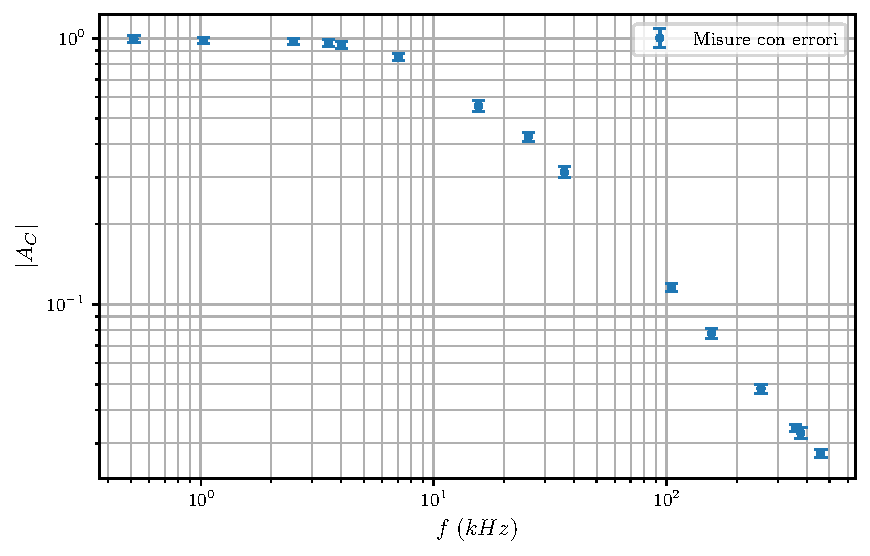
\includegraphics{onda_sin_AC(f).pdf}
%    \caption{Grafico logaritmico del modulo della funzione di trasferimento ai capi di $C$ in funzione di $f$}
%    \label{fig:funzione di trasferimento C}
%\end{figure}

%? \newpage

Si osserva che il modulo della funzione di trasferimento, in scala logaritmica, assume un andamento lineare agli estremi del grafico. A basse frequenze la funzione avrà andamento costante mentre ad alte frequenze si avrà un andamento lineare con pendenza $-1$.

\begin{figure}[ht!]
    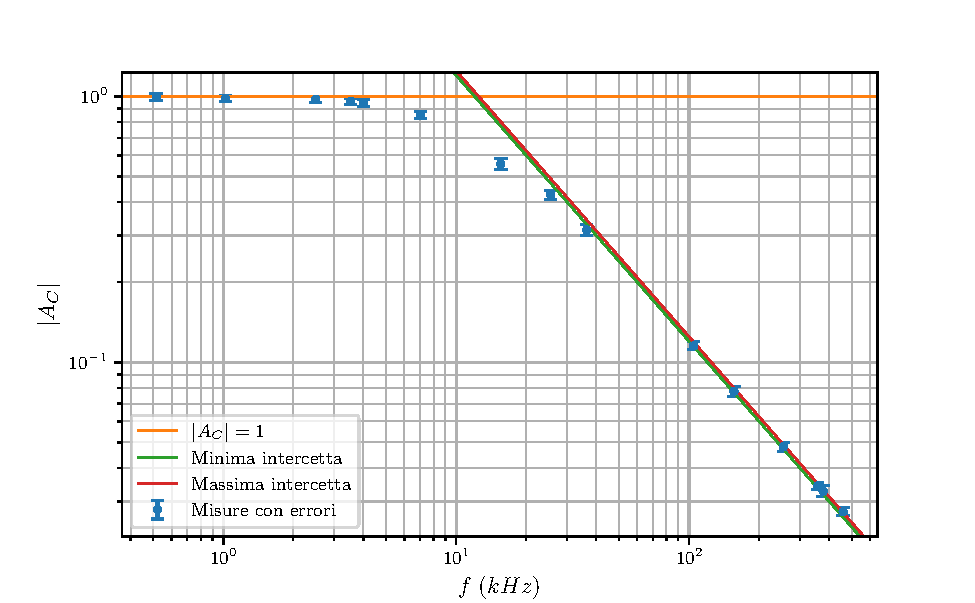
\includegraphics{onda_sin_AC(f)_taglio.pdf}
    \caption{Rette nelle zone di linearità del grafico del modulo della funzione di trasferimento ai capi di $C$}
    \label{fig:frequenza di taglio C}
\end{figure}

\begin{figure}[ht!]
    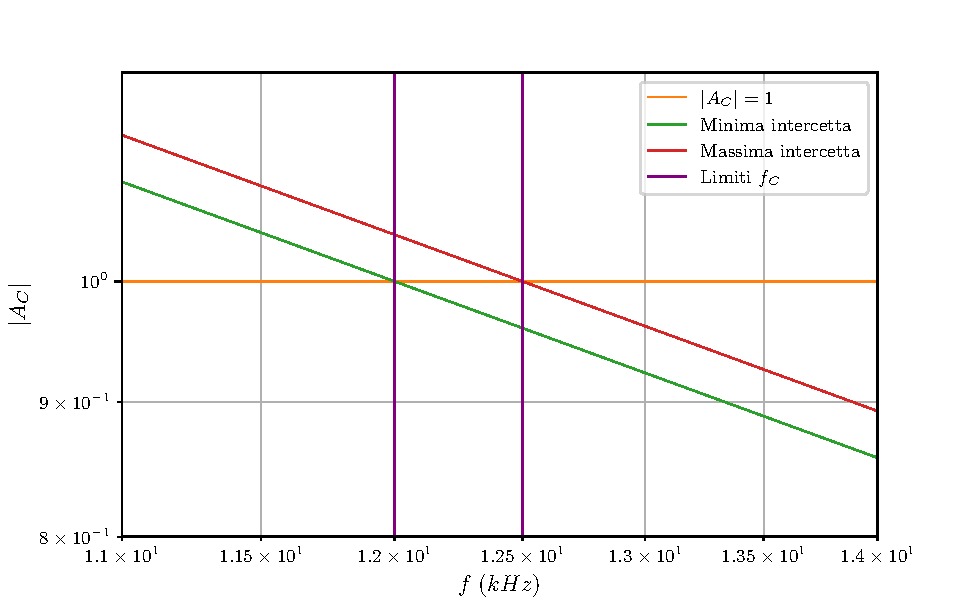
\includegraphics{onda_sin_AC(f)_taglio_frequenza.pdf}
    \caption{Zoom della \autoref{fig:frequenza di taglio C} per la stima della frequenza di taglio}
    \label{fig:frequenza di taglio C zoom}
\end{figure}

\newpage

Le rette si intersecano nei punti di frequenze

\begin{align*}
    f_{C \; min} &= 12.0 \; kHz \\
    f_{C \; max} &= 12.95 \; kHz
\end{align*}

\begin{align*}
    f_{C \; best} &= \frac{f_{C \; max} + f_{C \; min}}{2} = 12.475 \approx 12.5 \; kHz \\
    \delta f_{C} &= \frac{f_{C \; max} - f_{C \; min}}{2} = 0.475 \approx 0.5 \; kHz
\end{align*}

Quindi il valore della frequenza di taglio calcolata utilizzando le misure ai capi di $C$ è \(f_{C} = (12.5 \pm 0.5) \; kHz\).

Riportiamo le frequenze in \autoref{fig:fase C} per verificare che i valori della fase siano compatibili con la frequenza di taglio ottenuta.

\begin{figure}[ht!]
    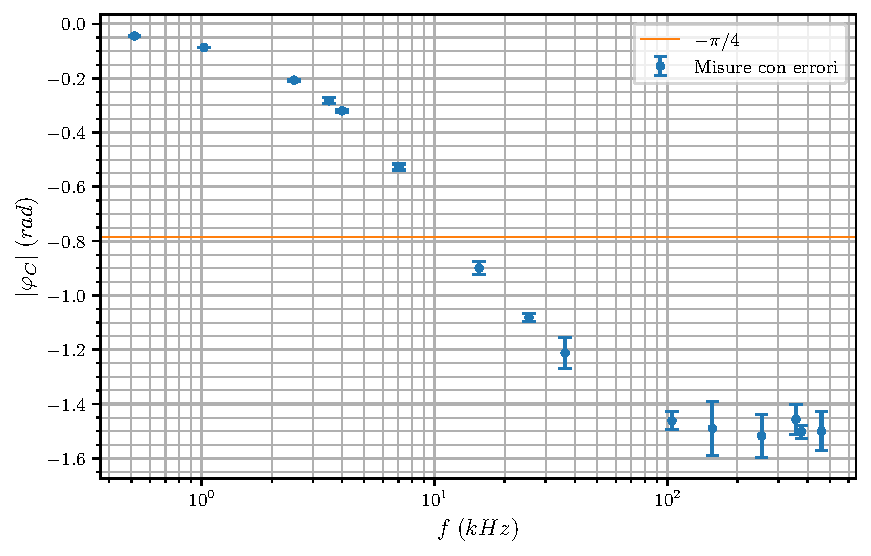
\includegraphics{onda_sin_phi(f)_C.pdf}
    \caption{Grafico della fase della funzione di trasferimento ai capi di $C$}
    \label{fig:fase C}
\end{figure}

Visto l'andamento decrescente della funzione, la frequenza di taglio risulta compatibile con i valori della fase.

\newpage

\subsection{Funzione di trasferimento ai capi di $R$}

\subsubsection{Dati ed errori}

Nella \autoref{tab:misure onda sinusoidale R} sono riportati i risultati delle misurazioni effettuate con i relativi errori. 

Per le tensioni in entrata $V_{in}$ la scala utilizzata è sempre di $1 V$ con errore $\delta V_{in} = 0.1 V$; questi non sono riportati in tabella per compattezza.

\begin{table}[ht!]
    \centering
    \caption{Misure dell'onda sinusoidale ai capi di $R$}
    \import{../tables/}{onda_sin_VR.tex}
    \label{tab:misure onda sinusoidale R}
\end{table}


\subsubsection{Analisi dati}

I valori del modulo e della fase della funzione di trasferimento ai capi di $R$ sono stati riportati nella \autoref{tab:funzione di trasferimento R}.

\begin{table}[ht!]
    \centering
    \caption{Modulo e fase della funzione di trasferimento ai capi di $R$}
    \import{../tables/}{funzione_di_trasferimento_R.tex}
    \label{tab:funzione di trasferimento R}
\end{table}

Riportando le misure della \autoref{tab:funzione di trasferimento R} in un grafico logaritmico $|A_{R}|(f)$ si ottiene la \autoref{fig:frequenza di taglio R}.

%? Nella funzione $|A_{R}|$ si avrà un andamento lineare a basse frequenze; quindi è stata tracciata una retta di pendenza $1$ passante per i punti situati all'estrema sinistra del grafico. Questa retta interseca l'asintoto orizzontale $|A_{R}| = 1$ alla frequenza di taglio $f_{R}$. 
%todo: ricopia quanto scritto @ riga 217

In maniera opposta alla funzione di trasferimento valutata ai capi di $C$, a basse frequenze la funzione avrà andamento lineare con pendenza $1$, mentre sarà costante per frequenze alte.

\begin{figure}[ht!]
    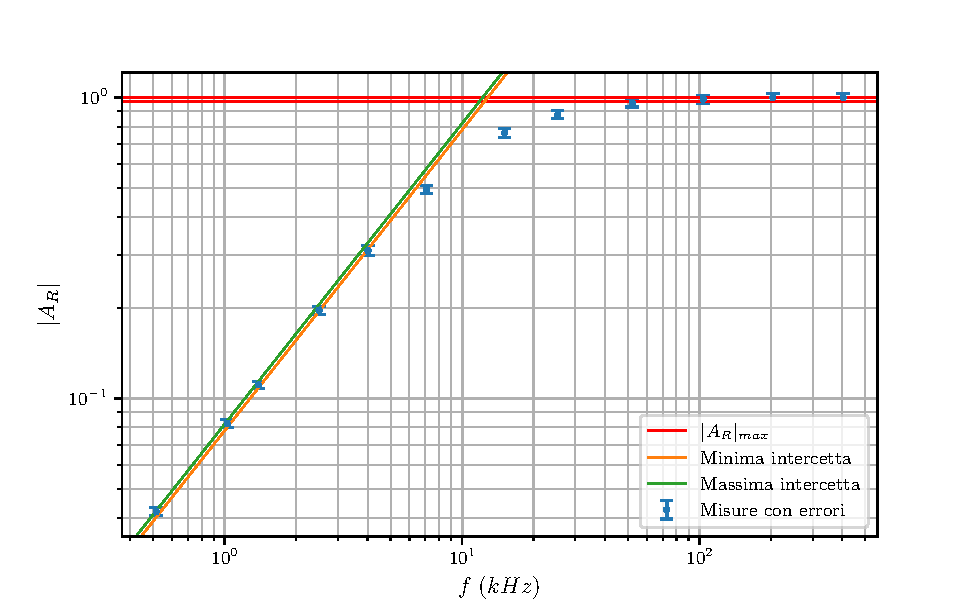
\includegraphics{onda_sin_AR(f)_taglio.pdf}
    \caption{Rette nelle zone di linearità del grafico del modulo della funzione di trasferimento ai capi di $R$}
    \label{fig:frequenza di taglio R}
\end{figure}

\newpage

\begin{figure}[ht!]
    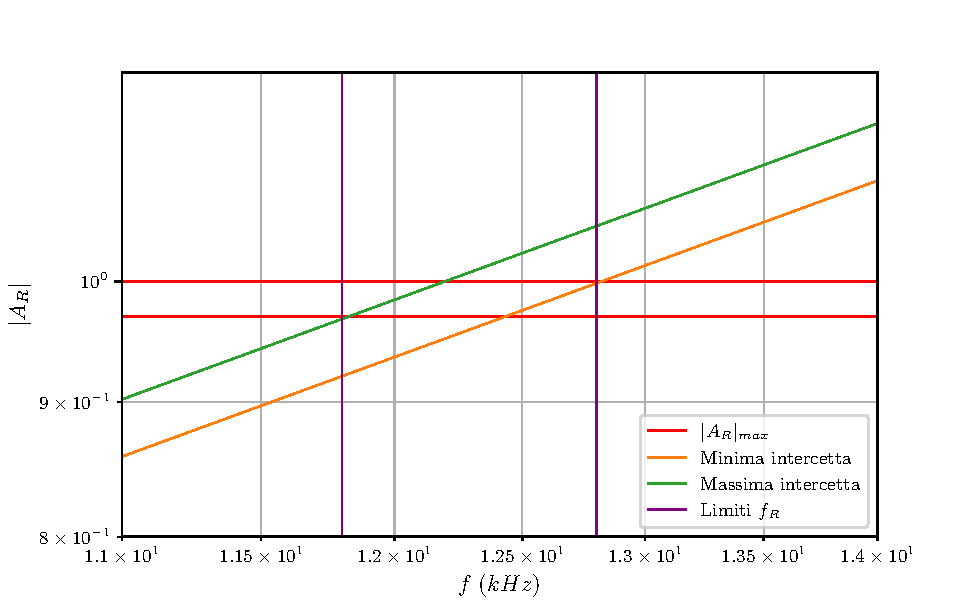
\includegraphics{onda_sin_AR(f)_taglio_frequenza.pdf}
    \caption{Zoom della \autoref{fig:frequenza di taglio R} per la stima della frequenza di taglio}
    \label{fig:frequenza di taglio R zoom}
\end{figure}

\begin{align*}
    f_{R \; min} &= 11.8 \; kHz \\
    f_{R \; max} &= 12.8 \; kHz
\end{align*}

\begin{align*}
    f_{R \; best} &= \frac{f_{R \; max} + f_{R \; min}}{2} = 12.3  \; kHz \\
    \delta f_{R} &= \frac{f_{R \; max} - f_{R \; min}}{2} = 0.5 \; kHz
\end{align*}

Quindi il valore di \(f_{R} = (12.3 \pm 0.5) \; kHz\).

Riportiamo le frequenze in \autoref{fig:fase R} per verificare che i valori della fase siano compatibili con la frequenza di taglio ottenuta.

\begin{figure}[ht!]
    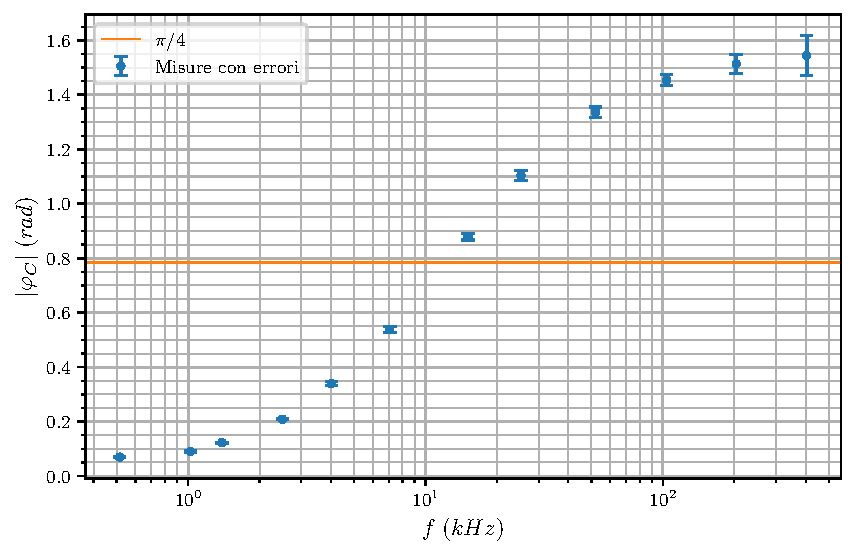
\includegraphics{onda_sin_phi(f)_R.pdf}
    \caption{Grafico della fase della funzione di trasferimento ai capi di $R$}
    \label{fig:fase R}
\end{figure}

Visto l'andamento decrescente della funzione, la frequenza di taglio risulta compatibile con i valori della fase.

\newpage

\section{Conclusioni}

Tramite il valore di $\tau = (13.5 \pm 0.7) \; \mu s$ ottenuto nella \autoref{sec:onda quadra} è possibile calcolare (\autoref{eq:f(tau)}) la frequenza di taglio del circuito $f_{\tau} = (11.8 \pm 0.6) \; kHz$.

\begin{align} \label{eq:f(tau)}
    \begin{split}
        f_{\tau} &= \frac{1}{2 \pi \tau} \\
        \delta f_{\tau} &= \frac{\delta \tau}{\tau} \; f
    \end{split}
\end{align}

Confrontando il valore appena ottenuto con $f_{C}$ ed $f_{R}$ essi risultano compatibili, come è possibile vedere nella \autoref{fig:fC ed fR compatibili}.

\begin{align*}
    f_{C} &= (12.5 \pm 0.5) \; kHz \\
    f_{R} &= (12.3 \pm 0.5) \; kHz
\end{align*}

\begin{figure}[ht!]
    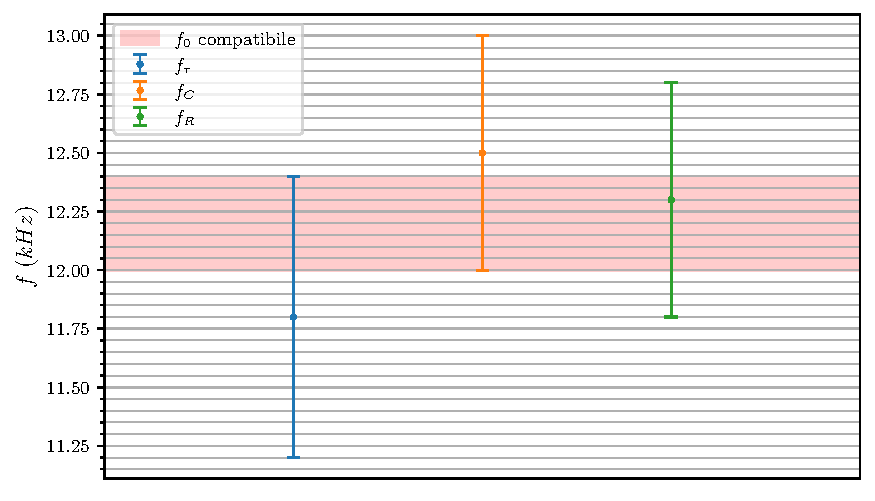
\includegraphics{f_0_compatibili.pdf}
    \caption{Verifica della compatibilità di $f_{C}$ ed $f_{R}$}
    \label{fig:fC ed fR compatibili}
\end{figure}

\newpage

È possibile dare un valore finale di $f_{0} = (12.2 \pm 0.2) \; kHz$.

\end{document}